% !TeX program = xelatex 

\PassOptionsToPackage{prologue, dvipsnames}{xcolor}
\documentclass[AutoFakeBold,AutoFakeSlant]{beamer}
\usetheme{metropolis}           % Use metropolis theme
\setbeamercovered{transparent}
\usepackage{listings}
\usepackage{grid-system}
\usepackage{ThinctPPT}
\usepackage[font=normalsize,labelfont=sf,textfont=sf]{subcaption} % Use only subcaption, not subfig

% 支持中文的设置
\usepackage{xeCJK}
\usepackage{fontspec}
\setCJKmainfont[ItalicFont=思源宋体,BoldFont=SourceHanSerifSC-Bold]{Source Han Serif SC}
\newcommand{\KaiTi}{\CJKfontspec{楷体}}%用命令\fzkaiti调用方正楷体简体

% other packages
\usepackage{latexsym,amsmath,xcolor,multicol,booktabs,calligra}
\usepackage{graphicx,pstricks,listings,stackengine}
\usepackage{wrapfig}
\usepackage[english]{babel}
\usepackage[font=normalsize,labelfont=sf,textfont=sf]{subcaption}


\title{\textbf{2023}\\年终总结}
\date{\today}
\author{\includegraphics[width=0.26\linewidth]{LaserMaker}\\软件部~/~王升平}

% 定义背景图片
%\usebackgroundtemplate{
%	
\includegraphics[width=\paperwidth,height=\paperheight]{bk}
%}

\usepackage{geometry}
\geometry{left=0.2cm,right=0.2cm,top=0cm,bottom=0cm}

\begin{document}
	
	\maketitle
	
	\section{过去一年}
	\subsection{进度数据}
	
	\begin{frame}[fragile]
		\LogoFrametitle{2023年度发现的BUG统计图表}
		\begin{figure}
			\centering % 将整个 figure* 居中
			\begin{subfigure}{\linewidth}
				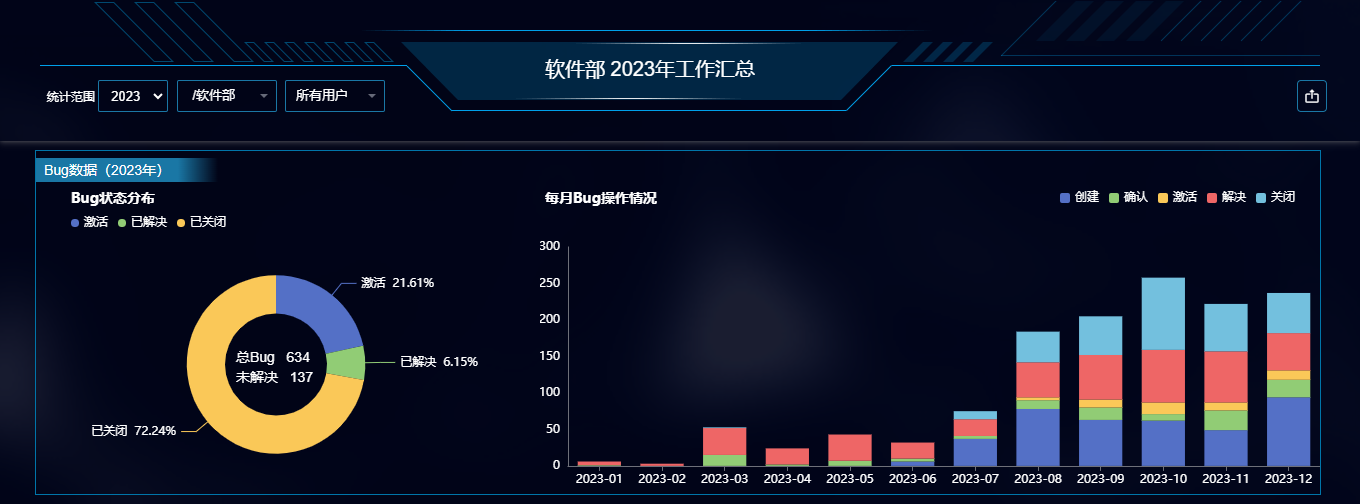
\includegraphics[width=\linewidth]{bug}
			\end{subfigure}
		\end{figure} 
		
		\begin{minipage}[l]{0.3\linewidth}
			\large
			总BUG数 : 634 \\
			未解决  : 137
		\end{minipage}\hfill
		\begin{minipage}[l]{0.6\linewidth}
			\footnotesize
			\linespread{1.5} \selectfont
			上半年主要程序刚发布,只做了一些简单的交互测试,发现的BUG较少.下半年产品用户越来越多,产品和用户以及自身的测试团队组建,一同发现BUG,导致BUG激增。
		\end{minipage}
	\end{frame}
	
	\begin{frame}[fragile]
		\LogoFrametitle{2023年度测试用例统计图表}
		\begin{figure}
			\centering % 将整个 figure* 居中
			\begin{subfigure}{\linewidth}
				\includegraphics[width=\linewidth]{Case}
			\end{subfigure}
			
			\begin{minipage}[l]{0.3\linewidth}
				\large
				通过率 : 87.18\% \\
				失败率 : 12.82\%
			\end{minipage}\hfill
			\begin{minipage}[l]{0.6\linewidth}
			\footnotesize
			\linespread{1.6} \selectfont
			上半年之前只有一个测试人员,并且兼做开发任务。下半年开始随着测试团队扩大,用户反馈增多,测试用例也越来越细化。
			\end{minipage}
		\end{figure} 
	\end{frame}
	
	\begin{frame}[fragile]
		\LogoFrametitle{2023年度开发任务统计图表}
		\begin{figure}
			\centering % 将整个 figure* 居中
			\begin{subfigure}{\linewidth}
				\includegraphics[width=\linewidth]{Task}
			\end{subfigure} 
			
			\begin{minipage}[l]{0.3\linewidth}
				\large
				总任务数 : 204 \\
				未完成  : 20
			\end{minipage}\hfill
			\begin{minipage}[l]{0.6\linewidth}
				\footnotesize
				\linespread{1.6} \selectfont
				上半年主要是程序的维护和准备发布阶段,任务主要在发布前后有激增.下半年主要随着团队人员增加,自九月份开始任务量逐渐形成递增态势.
			\end{minipage}
		\end{figure}
	\end{frame}
	
	\begin{frame}[fragile]
	\LogoFrametitle{2023年度用户量统计}
	\begin{figure}
		\centering % 将整个 figure* 居中
		\begin{subfigure}{\linewidth}
			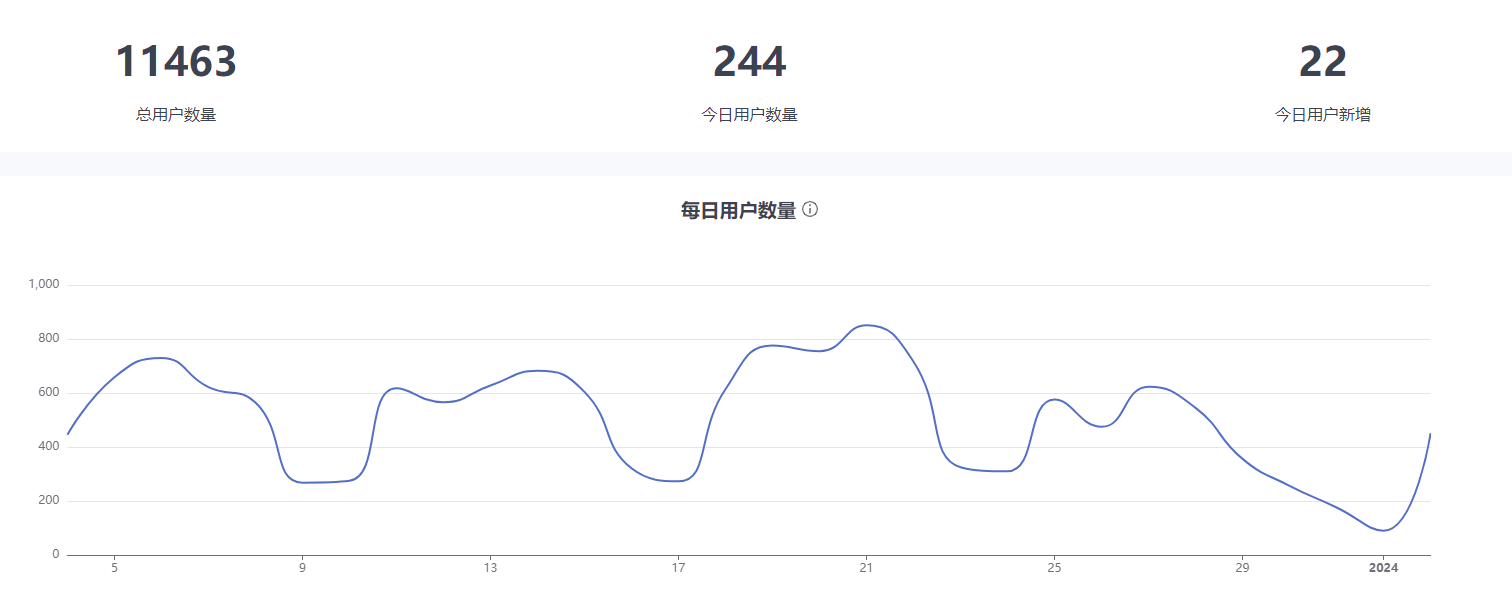
\includegraphics[width=\linewidth]{users_numbers}
		\end{subfigure} 
		
		\begin{minipage}[l]{0.3\linewidth}
			\large
			总用户数量:11463
		\end{minipage}\hfill
		\begin{minipage}[l]{0.6\linewidth}
			\footnotesize
			\linespread{1.6} \selectfont
			该数据只包含LaserMaker2.0自今年9月份至今的统计数据。
		\end{minipage}
	\end{figure}
	\end{frame}
	
	\begin{frame}[fragile]
		\LogoFrametitle{开发节点总结}
		\large
		\linespread{1.6}
		\selectfont
		\textbf{版本发布节奏:}
		\begin{quote}
			\textbf{每周}最后一天出一个\textbf{内部版本}{\tiny (12月底更新至:Alpha.28)}\\
			\textbf{每月}最后一天出一个\textbf{官网版本}{\tiny (12月底更新至:Beta.12)}
		\end{quote}
		
		\bigskip
		\bigskip
		
		\large
		\linespread{1.6}
		\selectfont
		\textbf{关键节点:}
		\begin{quote}
		\textbf{3.31} {\large 发布LaserMaker 2.0(Beta)} \\
		\textbf{8.01} {\large 提升复杂图元的操作流畅性体验} \\
		\textbf{8.31} {\large 在线收集程序崩溃文件} {\tiny (降准定位崩溃问题)} \\
		\textbf{12.26} {\large 降低内存消耗,进一步提升流畅性}{\tiny (将在20240131发布)} \\
		\textbf{12.31} 发布视觉业务模块
		\end{quote}
	\end{frame}
	
	\subsection{团队建设}
	\begin{frame}[fragile]
		\LogoFrametitle{团队建设}
		\large
		
		\footnotesize 
		\linespread{1.5} \selectfont
		\textbf{\large 开发组}
		\begin{quote}
			\begin{enumerate}
				\item 有效加快了细节需求的开发速度
				\item 加快了BUG维护进度
			\end{enumerate}
		\end{quote}
		
		\bigskip
		\bigskip
		
		\begin{minipage}[l]{0.5\linewidth}
			\footnotesize 
			\linespread{1.5} \selectfont
			\textbf{\large 算法组}\\
			\begin{quote}
				\begin{enumerate}
					\item 协助Bolt进行视觉之间工作,积累视觉经验
					\item 成功解决了图像操作中的轮廓提取等问题
				\end{enumerate}
			\end{quote}
		\end{minipage}\hfill
		\begin{minipage}[l]{0.5\linewidth}
			\footnotesize 
			\linespread{1.5} \selectfont
			\textbf{\large 测试组}\\
			\begin{quote}
				\begin{enumerate}
					\item 全面编写测试用例,覆盖多种使用场景。
					\item 每次发布之前,进行大规模的递归测试,保证解决过的问题不再出现。
				\end{enumerate}
			\end{quote}
		\end{minipage}
	\end{frame}
	
	
	\section{不足}
	\begin{frame}[fragile]
		\LogoFrametitle{认识不足}
		\large
		
		\begin{minipage}[l]{0.3\linewidth}
			\footnotesize 
			\linespread{1.5} \selectfont
			\textbf{\large 需求开发进度\\跟不上}\\
			成员经验还是有欠缺。另外,维护工作量吊车尾。
		\end{minipage}\hfill
		\begin{minipage}[l]{0.3\linewidth}
			\footnotesize 
			\linespread{1.5} \selectfont
			\textbf{\large 维护进度\\跟不上}\\
			随着测试越来越深入细致,用户量越来越多,BUG也成比例增多,需要进一步提升团队的专业技能
		\end{minipage}\hfill
		\begin{minipage}[l]{0.3\linewidth}
			\footnotesize 
			\linespread{1.5} \selectfont
			\textbf{\large 测试业务\\不够专业}\\
			只能进行表层的UI交互测试,不如专业用户的反馈。没有测试到点子上,导致程序在用户端才发现了诸多问题。
		\end{minipage}
	\end{frame}
	
	\section{未来工作计划}
	\subsection{团队业务技能培养}
	\begin{frame}[fragile]
		\LogoFrametitle{团队业务技能培养}
		\large
		\linespread{2.8} \selectfont
		\begin{enumerate}
			\item 继续做好推动各个负责人的工作进度
			{
				\item
				提高团队的业务能力
				\begin{enumerate}
					\item 分享修改BUG的经验
					\item 培训业务知识点
				\end{enumerate}
			} 
		\end{enumerate}
	\end{frame}
	
	\subsection{工作内容}
	\begin{frame}[fragile]
	\LogoFrametitle{工作内容}
	\large
	
	\begin{minipage}[l]{\linewidth}
		\footnotesize 
		\linespread{1.5} \selectfont
		\textbf{\large 测试组}
		\begin{enumerate}
			\item 自动化测试已完成部分部署,24年会开始统计其效果,进一步推进:达到自动化回归测试,减少测试人力成本,使其做更有挑战的白盒测试任务.
			\item 继续细化测试用例,贴近用户的常规操作,使用自动化工具完成UI交互点击功能,减少黑盒测试人力成本.
			\item 测试人员提升能力到编写测试脚本:黑盒和白盒.
		\end{enumerate}
	\end{minipage}
	
	\bigskip
	\bigskip
	
	\begin{minipage}[l]{0.45\linewidth}
		\footnotesize 
		\textbf{\large 开发组}\\
		继续培训基础知识,从根本解决问题,提升开发效率。\\
		24年的开发计划:
		\begin{enumerate}
			\item LaserMarker打标机
			\item 打通在线社区-浏览器
			\item 待定...
		\end{enumerate}
	\end{minipage}\hfill
	\begin{minipage}[l]{0.45\linewidth}
		\footnotesize 
		\textbf{\large 算法组}
		\begin{enumerate}
			\item 解决新品发布后,用户反馈的视觉模块问题
			\item 使用OpenCV代替Halcon,完成自主算法并跨平台.
		\end{enumerate}
	\end{minipage}
	\end{frame}
		
	\begin{frame}[fragile]
		\LogoFrametitle{汇报完毕}
		\begin{center}
			\Huge
			谢谢!
		\end{center}
	\end{frame}
\end{document}
